The AUC and prediction rate of predicting future cyber attacks using PLP on the data set described in \secref{cyberattacks} is shown in \figref{fig:plp_auc} for different lengths of the set used for testing.
\begin{figure}[!ht]
\centering
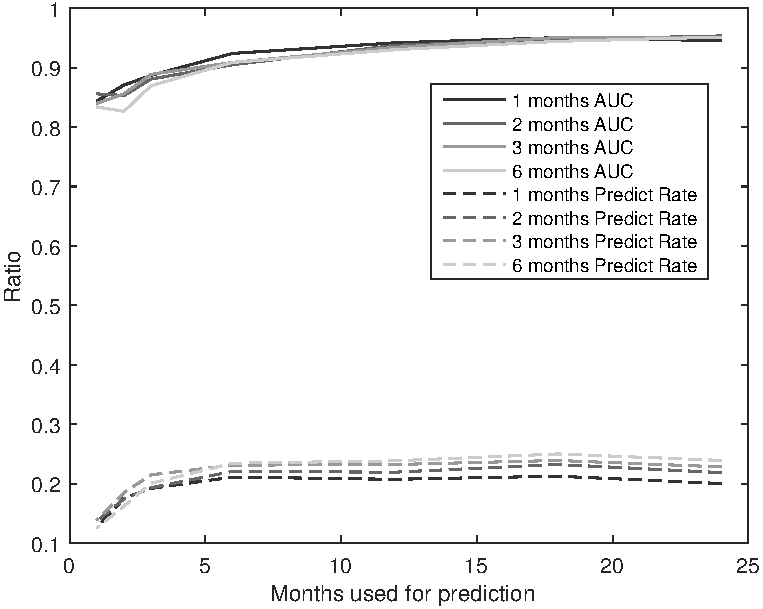
\includegraphics[scale=0.9]{images/auc_plp_result.pdf}
\caption{\label{fig:plp_auc} AUC and Prediction rate for the PLP algorithm used on the cyber attack bipartite graph. The different shades of grays represent differents length of time period used for testing (in months). AUC was calculated according to the description in section \ref{plp:auc} and prediction rate according to \ref{plp:predict_rate}.}
\end{figure}

How great the natural limitations of the algorithm are can be seen in \figref{fig:plp_max} where the maximum possible prediction rate, the ratio of cyber attacks with same actors as was previously seen in the prediction set and the ratio of cyber attacks that involved at least one new actor is presented.

\begin{figure}[!ht]
\centering
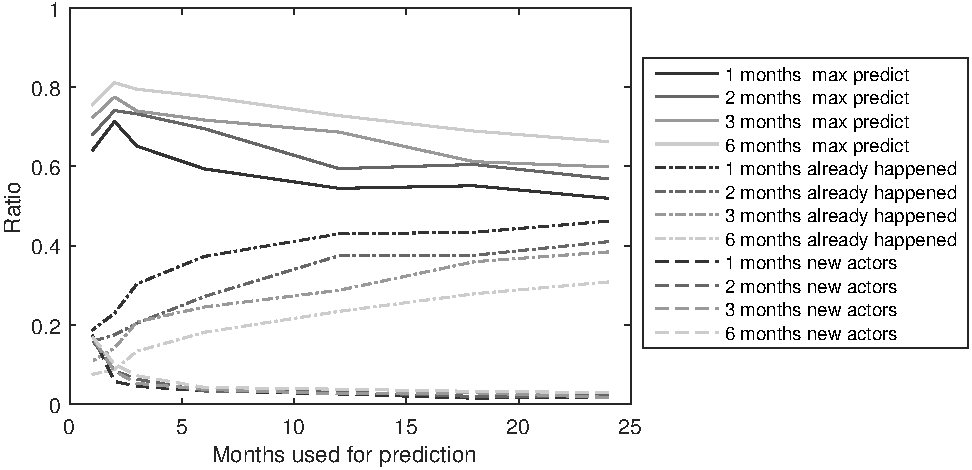
\includegraphics[width=\textwidth]{images/max_plp_result.pdf}
\caption{\label{fig:plp_max} 
Maximum prediction rate possbile for PLP for comarison with the prediction rate in \figref{fig:plp_auc}. Also showing the ratio of attacks with set of actors already in prediction set as well as the ratio of attacks involving at least one new actor.}
\end{figure}

We find that the auc increases around 10 percent units from 1 month of prediction data to 24 months of prediction data. However, the prediction rate does not vary that much for length of prediction data of at least 6 months.
